\documentclass[12pt]{article}
\usepackage[margin = 1in]{geometry}
\usepackage[USenglish]{babel}
\usepackage{natbib}
\usepackage{graphicx}
\usepackage{fancyhdr}
\usepackage{setspace}
\usepackage{amsmath}
\usepackage{lscape}
\usepackage{dcolumn}
\usepackage{xcolor}
\usepackage{subcaption}
\usepackage{enumerate}
\usepackage{longtable}
\usepackage{tabularx}
\usepackage{booktabs}
\usepackage{arydshln}
\usepackage{dcolumn}
\usepackage[colorlinks=true,citecolor=red!50!black,urlcolor=blue!50!black,linkcolor=red!50!black]{hyperref}


\author{Patrick W. Kraft\footnote{Assistant Professor, University of Wisconsin-Milwaukee, \href{mailto:kraftp@uwm.edu}{kraftp@uwm.edu}.
}}

\title{Change My View\\
\large{Do Moral Appeals Facilitate Compromise?}\footnote{The manuscript and code are available on GitHub: \url{https://github.com/pwkraft/cmv}.}}
%\large{Morally Congruent Arguments Facilitate Compromise}}
%\large{Morally Congruent Arguments Facilitate Persuasion}}
\date{}

% sans serif font
\renewcommand{\familydefault}{\sfdefault}

\begin{document}
\maketitle
\doublespacing
\thispagestyle{empty}

\begin{center}
-- WORK IN PROGRESS -- \\
PLEASE DO NOT CITE OR REDISTRIBUTE WITHOUT PERMISSION
\end{center} 

\hfill
\begin{abstract}\singlespacing
\noindent The American electorate is becoming increasingly polarized. According to research in moral psychology, these growing disagreements between liberals and conservatives can be attributed to fundamental differences in the moral frameworks that shape individual ideology. Indeed, scholars suggest that ideologues would be more likely to reach compromise if both sides spoke the same ``moral language.'' While this implicit assumption has intuitive appeal, it remains largely untested empirically. Drawing on a unique dataset from the online discussion board \emph{Reddit}, this paper examines how moral appeals can affect individual persuasion and the likelihood of compromise. %through deliberation.


\vspace{\baselineskip}
\noindent \textit{Keywords}: Moral Foundations, Conviction, Attitude Change, Persuasion, Compromise
\end{abstract}
\hfill

\newpage\setcounter{page}{1}
Recent years have witnessed a resurgence in partisan polarization in the United States. Politically engaged citizens hold more diverging policy
views, are more ideologically extreme, and exhibit stronger negative affect towards out-partisans than in the past \citep{hetherington2001resurgent, abramowitz2008polarization, iyengar2012affect, mason2014disrespectfully, huddy2015expressive, iyengar2015fear}. A growing literature in moral psychology---building on Moral Foundations Theory---attributes this divide (at least partially) to fundamental differences in moral frameworks that guide liberal and conservative thinking \citep[c.f.,][]{haidt2012righteous}. According to this perspective, liberals focus on \emph{individualizing} moral foundations, which include care/harm and fairness/cheating. Conservatives, on the other hand, also emphasize the remaining \emph{binding} foundations of loyalty/betrayal, authority/subversion, and sanctity/degradation \citep{haidt2007morality, graham2009liberals}. Differential emphasis on these moral dimensions is systematically related to attitudes towards a wide variety of divisive political issues \citep[e.g.][]{koleva2012tracing, kertzer2014moral, low2015moral}, personality traits like individual social dominance orientation (SDO) and right-wing authoritarianism (RWA) \citep{federico2013mapping}, as well as voting behavior \citep{franks2015using}. Overall, this body of research suggests that liberals and conservatives endorse different moral foundations and that these differences are related to political attitudes, evaluations, and behavior.

An important implicit assumption that has been made repeatedly in this literature is that liberals and conservatives would be more likely to come to agreements \emph{if only they focused on the same moral foundations}. For example \citet[365]{haidt2012righteous} concludes in his book \emph{The Righteous Mind: Why Good People Are Divided by Politics and Religion}: ``Once people join a political team, they get ensnared in its moral matrix. They see confirmation of their grand
narrative everywhere, and it's difficult---perhaps impossible---to convince them that they are wrong \emph{if you argue with them from outside of their matrix}'' (emphasis added). In an different article, \citet[1040]{graham2009liberals} contend that their findings ``help explain \emph{why liberals and conservatives disagree on so many moral issues} and often find it hard to understand how an ethical person could hold the beliefs of the other side: Liberals and conservatives \emph{base their moral values, judgments, and arguments on different configurations} of the five foundations.'' The underlying assumption that emphasizing the same foundations can facilitate compromise has important implications---especially in our current political environment. Somewhat surprisingly, however, it has never been subjected to a direct empirical test.

There are reasons to believe that compromise is still difficult---and potentially even further impeded---if individuals argue on the basis of the same set of moral foundations. \citet{skitka2005moral}, for example, provide a different theoretical perspective than MFT by conceptualizing moralization as a unique feature of attitude strength. According to this view, moral convictions are perceived as ``absolutes, or universal standards of truth that others should also share'' \citep[269]{skitka2010psychology}. As such, they combine the following attributes: they are viewed by individuals as applying to everyone (universality), they do not require an immediate underlying rationale but are rather seen as facts about the world (objectivity), they can be independent of authority and group norms (autonomy), they elicit strong emotional reactions, and they have an inherent motivational quality (motivation/justification) \citep{skitka2010psychology}. Building on this work, \citet{ryan2014reconsidering} argued that moral convictions are not restricted to issues that are traditionally perceived as ``moral,'' such as abortion or same-sex marriage, but can also include other issues such as economic policies. The degree of moral conviction may therefore vary between individuals as well as across issues. \citet{ryan2014reconsidering} further showed that the propensity to moralize---i.e.~the tendency to view an issue as a question of ``right and wrong''---is related to political participation, extreme political attitudes, arousal of negative emotions, and hostility. In a subsequent study, \citet{ryan2016no} suggested that moralization as a distinct characteristic of attitude intensity reorients behavior from maximizing gains to the general adherence to rules. Across multiple studies, the author showed that this tendency translates into stronger opposition to compromise about political issues and decreased support for compromising politicians. These patterns should also translate into attitudes towards---and interactions with---others who hold opposing views. Indeed, moral conviction has been shown to be related to stronger preferences for social distance from (and hostility towards) attitudinally dissimilar others and lower cooperativeness in groups holding heterogeneous views \citep{skitka2005moral}.

Ultimately, both perspectives in moral psychology lead to diverging expectations regarding the effect of moral appeals on persuasion and the likelihood of compromise: While moral foundations theory contends that agreement should be facilitated if two discussants focus on the same underlying foundations, the moral conviction literature suggests that any type of moral appeal should make it harder to overcome disagreement. The present paper tests both competing predictions by analyzing online discussions on the Reddit community \texttt{/r/ChangeMyView}. The following section discusses the data set in more detail. 

\section{Description of Dataset}\label{description-of-dataset}

\texttt{ChangeMyView} (CMV) is a Reddit community where participants begin a discussion by describing their opinion on a chosen issue in an original statement. Other participants are invited to challenge the original poster's (OP) arguments in order to change their view. The OP then responds to the arguments brought forward and explicitly identifies entries that changed his or her view by awarding a ``Delta'' (\(\Delta\)). For example, one original post that was added in 2014 (? check date again!) discusses the issue of marriage equality: 
\begin{quote}\singlespacing
\emph{CMV: I believe that the gay marriage discussion isn't as important as the media portrays it to be.}

The real problem is the concept of marriage itself. In my view, LGBT couples are already married, regardless of the legislation that is imposed on them. Marriage isn't a set of civil rights that confirms your connection to your partner, it's the choice you make to be in private, daily, lifelong commitment to another being.

Tradition dictates that in order to be `properly' married you have to exchange vows, get a ring, and have a massive celebration (the set of traditions change based upon the culture.) but marriage isn't that, it is simple commitment to another person. The main issue that gay marriage has is that not all couples are given the same civil liberties, but this does not mean that their marriages are void. marriage isn't decided by bystanders, it's decided by the people who live inside the union. It is for this very reason that a gay couple getting married doesn't affect your own marriage.

I've held this opinion for a while but have never had the opportunity to see if it stood up to criticism. CMV.
\end{quote}
Below is a sample response that lead the original author to award a \(\Delta\):
\begin{quote}\singlespacing
That would be true if it was just some odd tradition. But it isn't just the ceremony, but also a tax.

Right now there is a gay tax. Gay couples have to pay higher taxes than straight couples because the government gives a tax break for married couples. The reason for this is that married couples tend to be more efficient and better for the government. The government wants to encourage marriage, so as with all things they encourage they subsidize it.

Gay people provide the exact same benefits to marriage, if not more! Adoption being the largest one.

[\hspace{.2em}$\cdots$]

This tax comes through in multiple ways. The yearly tax and through inheritance. The government doesn't tax inheritance as much for marriage, but if they are simply partners then they get taxed when their ``partner'' dies.

The state also doesn't allow for gay couples see their loved ones in hospitals or prison because they aren't married.

If this was just in the church I wouldn't care. But this is much more than that."
\end{quote}
The participation rules of the community foster civil exchange of arguments---even for decisive issues---and OP's are encouraged to award \(\Delta\)s genuinely. As such, it provides a perfect opportunity to examine the role of moral appeals in persuasion and agreement.

\citet{tan2016winning} analyzed the discussion dynamics on \texttt{ChangeMyView} by focusing on language features that predict persuasiveness of discussion contributions as well as the malleability of original posts. The authors extract argument pairs that respond to an original post with only one being successful in changing the OPs view while being relatively similar in terms of their word choice.

{[}Elaborate on argument pair selection etc.{]}

The analyses reported below use the same data and case selection that was published by \citet{tan2016winning} as well as the Moral Foundations Dictionary proposed by \citet{graham2009liberals}.


\begin{figure}
\centering
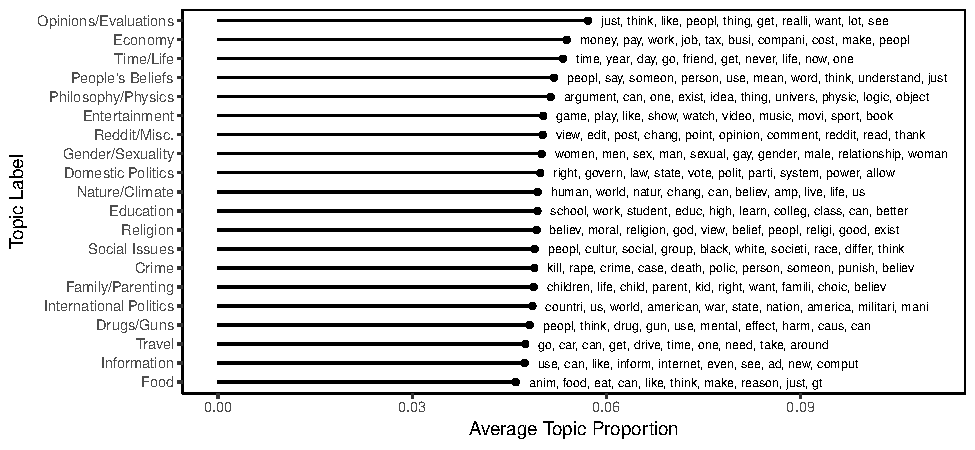
\includegraphics{/data/Dropbox/Uni/Projects/2017/cmv/calc/fig/topics.pdf}
\caption{Average topic proportions in original posts on \texttt{/r/ChangeMyView/}. Figure displays the five most likely terms associated with each respective topics.}
\end{figure}


\begin{figure}
\centering
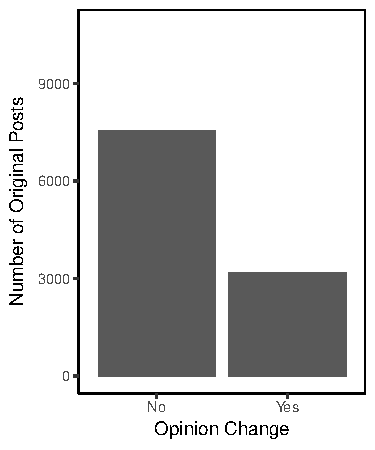
\includegraphics{/data/Dropbox/Uni/Projects/2017/cmv/calc/fig/delta.pdf}
\caption{Number of original posts on \texttt{/r/ChangeMyView/} that resulted in opinion change ($\Delta$ awarded by author) versus not.}
\end{figure}


\section{Moral Foundations and Persuadability}\label{moral-foundations-and-persuadability}

This figure shows that OPs who use fewer moral words in their opening statements are more likely to provide a \(\Delta\) in the subsequent discussion. This basic result is consistent with the moral conviction literature.

\begin{figure}
\centering
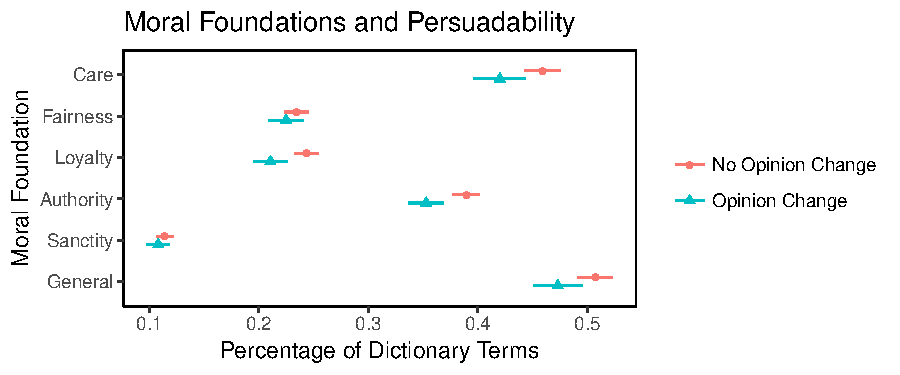
\includegraphics{/data/Dropbox/Uni/Projects/2017/cmv/calc/fig/persuadability.pdf}
\caption[Moral Foundations and Persuadability]{Moral Foundations and Persuadability: Average percentage of dictionary terms relative to the total number of words in each original post starting a discussion, comparing original posts where the author subsequently awarded a $\Delta$ (opinion change) or not (including 95\% confidence intervals).}
\end{figure}

\section{Is Moral Consistency
Convincing?}\label{is-moral-consistency-convincing}

Next, I examine the persuasiveness of moral arguments made within discussion contributions as a response to original posts that rely on any of the moral foundations.

\begin{figure}
\centering
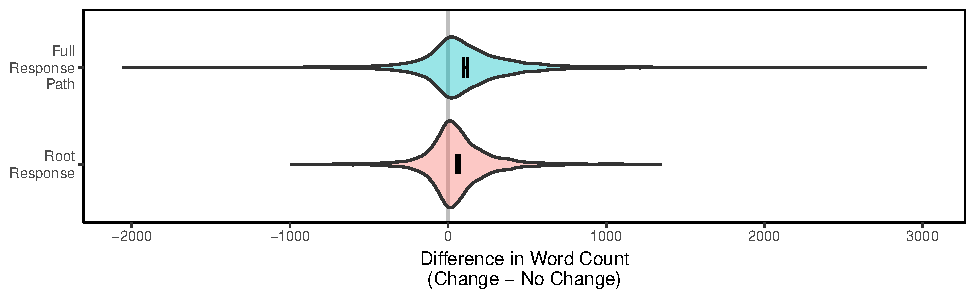
\includegraphics{/data/Dropbox/Uni/Projects/2017/cmv/calc/fig/wordcount_violin.pdf}
\caption{Something something.}
\end{figure}

\begin{figure}
\centering
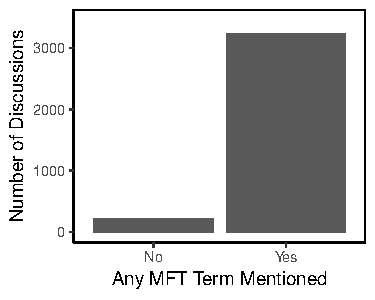
\includegraphics{/data/Dropbox/Uni/Projects/2017/cmv/calc/fig/mft_op_all.pdf}
\caption{Something something.}
\end{figure}



\begin{figure}
\centering
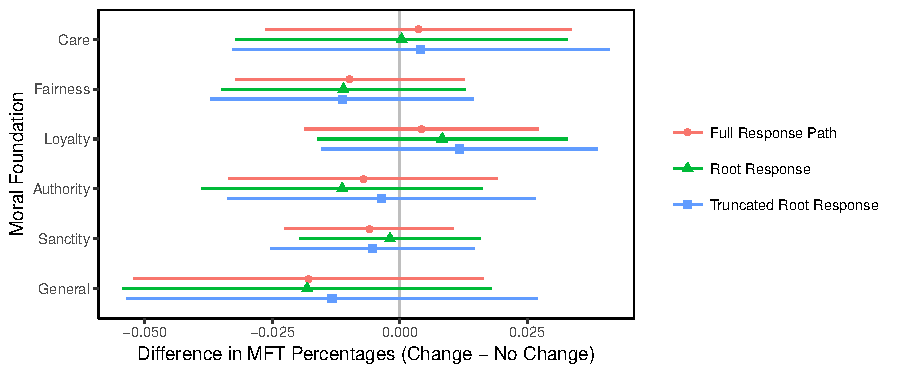
\includegraphics{/data/Dropbox/Uni/Projects/2017/cmv/calc/fig/persuasiveness.pdf}
\caption[Moral Foundations and Persuasiveness]{Moral Foundations and Persuasiveness: Average difference of dictionary term percentages relative to the total number of words in each original post starting a discussion, comparing original posts where the author subsequently awarded a $\Delta$ (opinion change) or not (including 95\% confidence intervals).}
\end{figure}



\begin{figure}
\centering
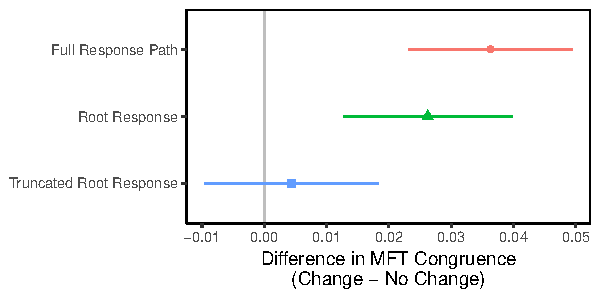
\includegraphics{/data/Dropbox/Uni/Projects/2017/cmv/calc/fig/cosine.pdf}
\caption{Yay, effects.}
\end{figure}





\section{Test measure of moral consistency}\label{test-measure-of-moral-consistency}


Consistency in moral appeals is larger in persuasive than non-persuasive arguments.

\section{Conclusion}\label{conclusion}

The preliminary results are consistent with the literature on moral conviction and clearly contradict the implicit assumptions made in the Moral Foundations literature. Overall, arguments that revolve around the same moral foundations are less likely to be persuasive. In most cases, moral appeals of any type appear counterproductive in facilitating compromise and changing people's minds.

% TO DOs, future directions, etc.:
% - examine specific topics (e.g., climate change etc.
% - clean original posts (links etc)
% - adjust confidence intervals to correct for multiple comparisons
% - improve code documentation, add comments in internal functions
% - check MFT scores in argument pairs (as well as OP entry)


% LIST for appendix:
% - distribution of response lengths
% - 

% TODO: implement John's feedback!

\clearpage
\singlespacing
\bibliographystyle{/data/Dropbox/Uni/Lit/apsr2006}
\bibliography{/data/Dropbox/Uni/Lit/Literature}

\end{document}